% CVPR 2027 submission DRAFT (generated 2026-10-11). Swap \documentclass/preamble for the official cvpr.sty template before submission.
% Conventions: \todo{} = missing result or check;  \verify{} = citation/venue to verify against the PDF.
\documentclass[10pt,twocolumn,letterpaper]{article}
\usepackage[margin=0.75in]{geometry}
\usepackage{times,graphicx,booktabs,amsmath,amssymb,xcolor,multirow}
\usepackage[numbers,sort&compress]{natbib}
\usepackage[hidelinks]{hyperref}
\newcommand{\todo}[1]{\textcolor{red}{[TODO: #1]}}
\newcommand{\verify}[1]{\textcolor{orange}{[verify: #1]}}
\title{Whoever Zooms Decides: Evidence Selection Is an Attack Surface\\for Gigapixel and High-Resolution Vision Models}
\author{Anonymous CVPR submission}
\date{}
\begin{document}
\maketitle

\begin{abstract}
Images that are too large to process at once are increasingly answered from a \emph{selected} subset: multiple-instance learning (MIL) models classify whole-slide images from their top-attended patches, and ``thinking-with-images'' agents answer high-resolution questions from the crops they zoom into.
We study the component everyone trusts and nobody audits: the selector.
Holding the image and the answering model fixed and changing only which evidence is shown, we find that the selector largely decides the answer.
On CAMELYON16, an adversarial selector drives attention top-$K$ MIL from 0.97 to 0.00 balanced accuracy; on breast-cancer biomarker prediction (BCNB), \emph{non-adversarial} selectors already flip 9--61\% of slide decisions and black-box transferred selectors flip 64--68\% ($K{=}8$).
On V*-Bench and HR-Bench, a single adversarial crop flips 64--70\% of answers of Qwen2.5-VL and Qwen3-VL even when the full image is visible at reduced resolution, and the models' own natural zooms flip 15--47\%.
As a remedy for the setting where the decider can only afford to inspect $K$ items and the readers are untrusted, we evaluate two-sided evidence debate~\cite{irving2018debate}: two selectors argue for opposite answers by revealing evidence to a question-blind judge.
Debate recovers 0.90--0.98 balanced accuracy on CAMELYON16 from a single surviving tumor patch up to 20\% tumor, against greedy and look-ahead liars, while a selector-free random-mask ensemble only catches up when evidence is dense; on VQA, training-free crop debate reaches 0.72--0.86, matching the model's own honest zoom.
\end{abstract}

%=====================================================================
\section{Introduction}
Gigapixel pathology slides ($\sim\!10^4$--$10^5$ patches) and 4K/8K photographs exceed what a model can process at full resolution. The dominant answer is \emph{selection}: an attention module keeps the top-$K$ patches~\cite{ilse2018abmil}, a retrieval step picks question-relevant regions, or an agent calls a zoom tool and answers from the crop~\cite{wu2024vstar,zheng2025deepeyes}. Selection is now the interface between the image and the decision.

This creates an unexamined trust assumption. Benchmarks audit the \emph{answerer}; the \emph{selector} is treated as a neutral pre-processing step. But if the answer is computed from what the selector shows, then whoever controls the selector, whether an adversary, a biased retrieval model, or the agent's own confirmation loop, controls the answer.

\paragraph{This paper measures that control and evaluates a defense.}
\begin{itemize}
\item \textbf{Threat (Sec.~\ref{sec:threat}).} With features, judge and image held fixed, we swap only the selector. Adversarial selectors drive MIL to $\approx$0 balanced accuracy on CAMELYON16 and BCNB; natural selectors (k-means coverage, question-relevance retrieval, hypothesis-confirming retrieval, independent models' attention) already flip 9--61\% of decisions; and one adversarial crop flips 64--70\% of VLM answers on V* and HR-Bench, with the models' own zooms flipping 15--47\%.
\item \textbf{Defense (Sec.~\ref{sec:debate}).} We instantiate Irving et al.'s debate~\cite{irving2018debate} for gigapixel MIL and VLM zoom: two debaters reveal $K$ patches or crops each, and a judge that never sees the full input decides. Debate is accurate \emph{and} robust at every evidence sparsity we test, whereas cooperative selectors are accurate but steerable and selector-free random masking is robust but only accurate when evidence is dense (Fig.~\ref{fig:sparsity}).
\item \textbf{Scope (Sec.~\ref{sec:discussion}).} Debate is not a compute saving: our debaters read the whole slide, and at equal compute debate ties a trusted full read. Its value is for deployments where the decider (a clinician, an expensive VLM, a regulator) inspects only $K$ items and the readers are not trusted. Its advantage over selector-free reading grows as evidence becomes sparser, and vanishes on diffuse labels (BCNB), as predicted.
\end{itemize}

%=====================================================================
\section{Related work}
\paragraph{Selection in MIL.} BagShift~\cite{bagshift2026} measures how non-adversarial patch selection changes MIL outputs on CAMELYON16 and PANDA; we share its paired protocol but add adversarial and question/hypothesis-conditioned selectors, VLM agents, and a defense. Pixel-level adversarial attacks on MIL and pathology CNNs~\cite{mil_adv2022,foote2021now} perturb inputs rather than selection. Evidence-sufficiency work (FOCI, GCE-MIL, ReaMIL, CAR-MIL)~\cite{foci2026,gcemil2026,reamil2026,carmil2026} asks which subsets suffice; we ask who chooses them. BEACON~\cite{beacon2026} argues relevance retrieval picks non-discriminative patches.
\paragraph{Zoom agents.} V*~\cite{wu2024vstar}, ViCrop~\cite{zhang2025vicrop}, DeepEyes~\cite{zheng2025deepeyes}, Mini-o3~\cite{minio3} and others zoom before answering. ViEBench~\cite{viebench2026}, Pinpoint-Bench~\cite{pixeleyes2026} and Distract-Bench~\cite{distract2026} audit grounding non-adversarially. MED~\cite{med2026} finds that tool-use RL mostly reduces tool-induced harm rather than learning to use crops; it does not substitute or attack crops. We control the crop directly.
\paragraph{Debate and prover--verifier games.} Debate was proposed with an MNIST sparse-pixel judge~\cite{irving2018debate}; Merlin-Arthur classifiers~\cite{waldchen2024merlin} and the Neural Concept Verifier~\cite{ncv2026} give soundness guarantees for prover/adversary feature selection; prover--verifier games~\cite{anil2021pvg,kirchner2024pvg,hammond2025nip} and LLM debate~\cite{khan2024debate,kenton2024scalable} study the text setting. Multimodal debate has been used with a blind text judge~\cite{adhikari2025debating} and for deception monitoring~\cite{fang2026debateimages}. A public report found that image-cell debate barely beats a random-mask judge ensemble~\cite{quantilized_debate}; we show this depends on evidence sparsity. We do not claim the debate mechanism; we claim its evaluation as a selector-robust protocol at gigapixel scale and on VLM zoom.

%=====================================================================
\section{Setup}\label{sec:setup}
\paragraph{Selected-evidence decision.} An input $x$ is a set of items $\{x_i\}_{i=1}^N$ (patches or tiles). A selector $S$ returns $K\!\ll\!N$ indices; a judge $J$ answers from $\{x_i\}_{i\in S(x)}$ (optionally with a low-resolution overview). We fix $x$ and $J$ and vary $S$.
\paragraph{Selectors.} (i) \emph{Deployed}: the judge's own attention top-$K$, or the VLM's own grounding zoom. (ii) \emph{Natural}: independent-model attention, instance-classifier scores, k-means coverage, question-relevance retrieval, hypothesis-conditioned retrieval, and agent loops. (iii) \emph{Adversarial}: white-box greedy selection towards a target answer, black-box transfer from a surrogate, and look-ahead (rollout) selection.
\paragraph{Debate.} Two debaters are assigned opposite answers and alternately reveal $K$ items each (greedy on exact incremental judge logits; a look-ahead liar optimizes over rollouts). The judge sees the revealed items with a presenter flag but not the question-specific full input. MIL judge: gated ABMIL~\cite{ilse2018abmil} on frozen features, trained on random-$K$ subsets, warm-started on attention-top-$K$ subsets for extreme sparsity. VLM judge: the same VLM, shown the global view and both crops; no training.
\paragraph{Data.} CAMELYON16~\cite{c16} (UNI~\cite{uni} features, 512px level-0 patches, 270 train / 129 test, 49 tumor); BCNB~\cite{bcnb} ER/PR/Grade-3 (CONCH~\cite{conch} features, 5-fold CV); V*-Bench~\cite{wu2024vstar} (191 questions) and HR-Bench-4K~\cite{hrbench} (200 questions, answer positions rotated); judges Qwen2.5-VL-7B~\cite{qwen25vl} and Qwen3-VL-8B~\cite{qwen3vl}; zoom agent DeepEyes-7B~\cite{zheng2025deepeyes}. Metric: balanced accuracy (MIL) and accuracy (VQA); MIL results are mean$\pm$sd over 3 seeds.
\paragraph{Sparsity intervention.} To control the evidence fraction on CAMELYON16 we (a) \emph{cap} each tumor slide to $t\in\{1,4,16,64\}$ tumor patches, dropping other tumor patches and their 8-neighbours, or (b) \emph{densify} by subsampling normal tissue so tumor is $\ge$5\% or 20\% (minimum bag 64). Train and test are treated identically.

%=====================================================================
\section{The selector decides}\label{sec:threat}
\begin{table}[t]\centering\small
\caption{\textbf{CAMELYON16, natural regime} (balanced accuracy, mean$\pm$sd, 3 seeds). Full-slide ABMIL: 0.969. Every cooperative selector is driven to $\approx$0 by an adversary; debate is not.}\label{tab:c16}
\setlength{\tabcolsep}{3pt}
\begin{tabular}{@{}lcccccc@{}}\toprule
$K$ & attn & attn (att.) & V-IP (att.) & liar cons. & rand-mask & debate\\\midrule
2  & .974 & .021 & .000 & .000 & .556 & \textbf{.943}$\pm$.023\\
4  & .978 & .000 & .000 & .000 & .628 & \textbf{.949}$\pm$.010\\
8  & .984 & .000 & .000 & .000 & .628 & \textbf{.971}$\pm$.011\\
16 & .978 & .000 & .000 & .000 & .703 & \textbf{.958}$\pm$.008\\\bottomrule
\end{tabular}\end{table}

\begin{table}[t]\centering\small
\caption{\textbf{Natural selectors already steer MIL} (BCNB-ER, ABMIL top-$K$ judge, $K{=}8$). Flip = fraction of slides whose decision differs from the deployed own-attention decision.}\label{tab:natural}
\begin{tabular}{@{}lcc@{}}\toprule
selector & BA & flip\\\midrule
own attention top-$K$ (deployed) & .758 & --\\
independent model's attention & .741 & .091\\
k-means coverage & .635 & .266\\
question-relevance retrieval & .613 & .177\\
random (mean of 32) & .651 & .230\\
confirm majority hypothesis & .525 & .232\\
confirm minority hypothesis & .581 & .608\\\midrule
black-box transfer (indep.\ full-slide surrogate) & .240 & .642\\
transfer from TransMIL surrogate & .110 & .681\\
white-box greedy & .020 & .784\\\bottomrule
\end{tabular}\end{table}

\paragraph{MIL.} Tab.~\ref{tab:c16}: with the judge, features and slide fixed, an adversarial selector reduces attention top-$K$, a V-IP querier~\cite{chattopadhyay2023vip} and a single-prover consultant to $\approx$0 at every $K$. The attack transfers: selectors optimized against an independent surrogate still drive BCNB-ER to 0.11--0.24 (Tab.~\ref{tab:natural}). More importantly, \emph{non-adversarial} selectors already change 9--61\% of decisions; a retrieval step that seeks evidence for a hypothesis flips 61\% when the hypothesis is the minority class. The same pattern holds for BCNB-PR/Grade-3 and a TransMIL judge \todo{appendix table}.

\paragraph{VLM zoom.} Tab.~\ref{tab:vlm}: on V* and HR-Bench, a single adversarial tile shown with a 768$^2$ global view flips 64--70\% of answers; a targeted attacker forces a \emph{chosen} wrong option 34--55\% of the time. Without an attacker, the set of natural zooms (the model's own grounding box and confirmation zooms for each option) contains an answer-flipping crop for 15--47\% of questions. The selector, not the image, is the bottleneck of these pipelines.

\begin{table}[t]\centering\small
\caption{\textbf{VLM zoom} (accuracy; flips = fraction of questions). Adversarial tiles chosen from exact option log-probs; debate is 1v1 crop debate with the global view, min over speaking order.}\label{tab:vlm}
\setlength{\tabcolsep}{3pt}
\begin{tabular}{@{}lccc@{}}\toprule
 & \multicolumn{2}{c}{V*} & HR-4K\\
 & Qwen2.5 & Qwen3 & Qwen2.5\\\midrule
full image, high-res & .707 & .743 & .590\\
global view only & .665 & .691 & .600\\
+ own grounding zoom$^\dagger$ & .824 & .875 & .718\\
+ GT tile & .838 & .838 & --\\\midrule
some adversarial tile flips (+global) & .639 & .702 & .625\\
targeted attack success (+global) & .518 & .551 & .342\\
some natural zoom flips & .267 & .152 & .470\\\midrule
\textbf{crop debate} (+global) & \textbf{.791} & \textbf{.859} & \textbf{.720}\\\bottomrule
\end{tabular}\\[2pt]
{\footnotesize $^\dagger$on questions where the box parsed (160/191, 160/191, 177/200).}
\end{table}

\paragraph{RL-trained zoom agents.} We run DeepEyes-7B~\cite{zheng2025deepeyes} with its official protocol (tool schema, greedy decoding; generation stopped at \texttt{</tool\_call>} as in its RL environment) and replace the crop service: every tool call returns an adversarial tile (top-4 by Qwen2.5-VL surrogate margin, black-box), a random tile, or the ground-truth tile. Tab.~\ref{tab:deepeyes}: the agent calls the tool on every question, yet its answer barely depends on what the tool returns. The ground-truth crop adds $\le$2.6 points even when the overview is only 768$^2$, and adversarial crops flip 3.1\% of correct answers (random: 1.3--1.5\%). Transcripts state ``the zoom-in confirms \ldots'' for crops that do not contain the object. This complements MED~\cite{med2026} with a causal test, and gives the second regime of our analysis: a zoom that carries the answer (Qwen with a crop: +15--17 points from the GT tile, 64--70\% flips) is both useful and attackable; a decorative zoom is neither.

\begin{table}[t]\centering\small
\caption{\textbf{DeepEyes-7B crop substitution} (V*, 191 questions). Flips are among natively-correct answers.}\label{tab:deepeyes}
\begin{tabular}{@{}lcc@{}}\toprule
overview given to the agent & full-res & 768$^2$\\\midrule
native (real crops) & .832 & .681\\
GT crop substituted & .838 & .707\\
adversarial crop substituted & .822--.827 & .675--.691\\
random crop substituted & .838--.843 & .696--.707\\\midrule
flipped by some adversarial crop & .031 & .031\\
flipped by some random crop & .013 & .015\\\bottomrule
\end{tabular}\end{table}

%=====================================================================
\section{Debate as a selector-robust protocol}\label{sec:debate}
\begin{figure*}[t]\centering
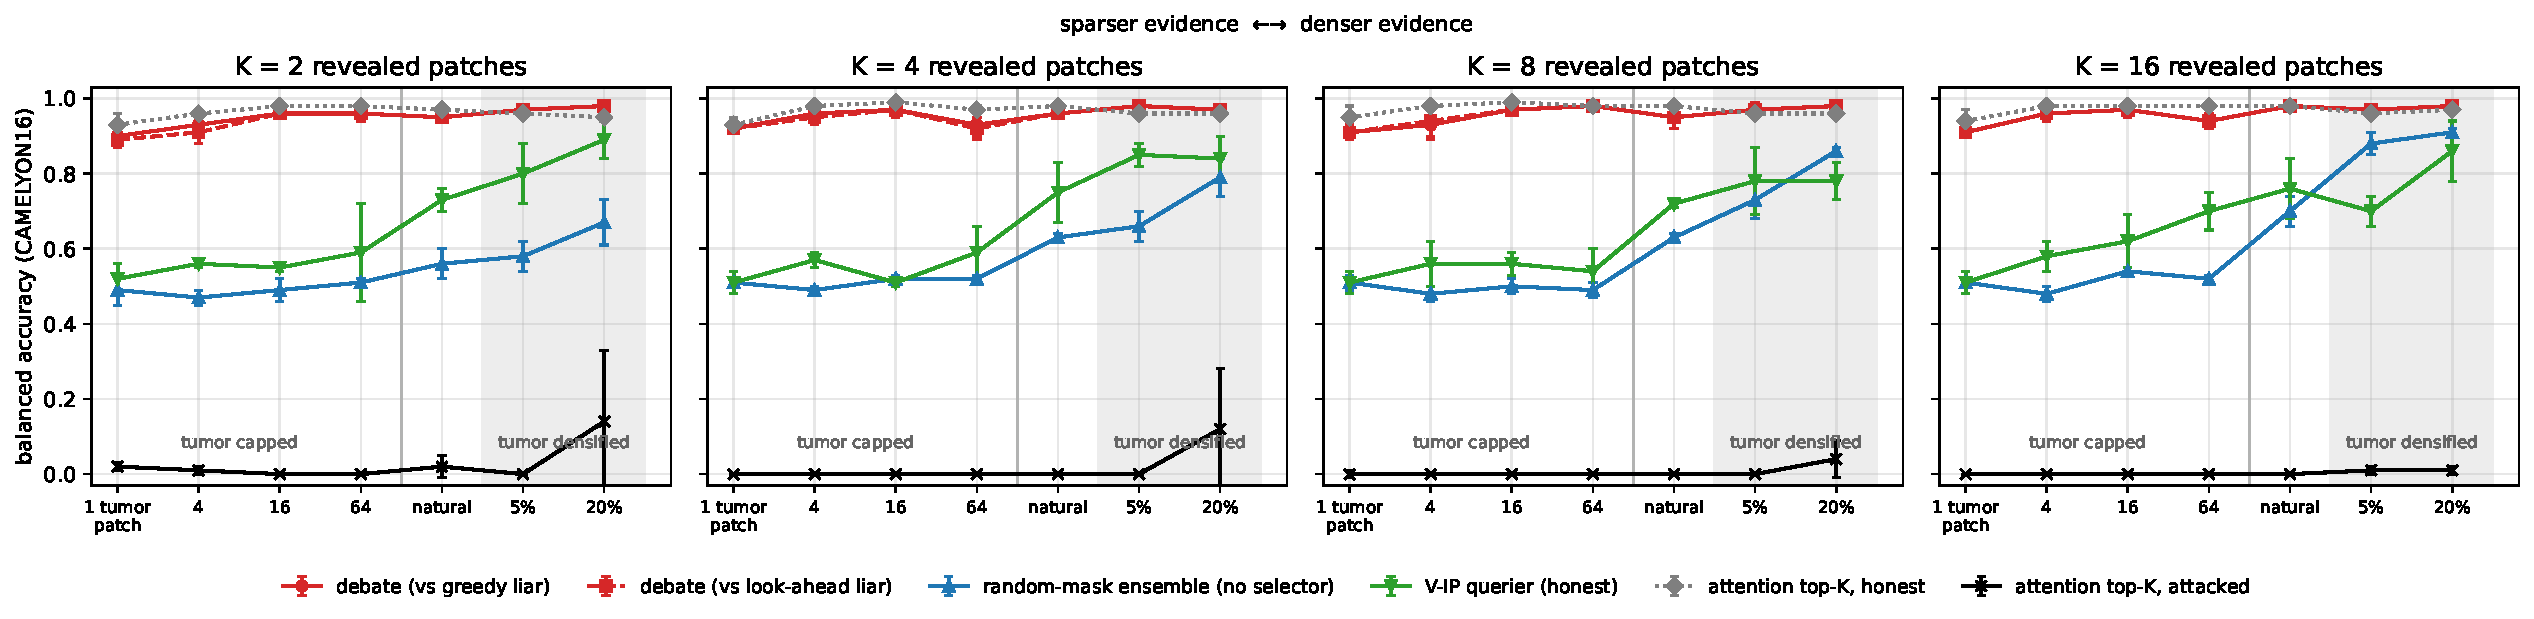
\includegraphics[width=\linewidth]{figs/fig_sparsity.pdf}
\caption{\textbf{Accuracy vs.\ evidence sparsity} (CAMELYON16, 3 seeds). Left of each panel: tumor capped to 1--64 patches; right: tumor densified to 5\%/20\%. Debate (red) stays at 0.90--0.98 against greedy and look-ahead liars. Selector-free random masking (blue) is robust but only accurate when evidence is dense. Cooperative selectors (grey, green) are accurate but collapse to $\approx$0 under attack (black).}\label{fig:sparsity}
\end{figure*}

\paragraph{Main result.} Debate is the only selected-evidence method that is both accurate and robust across sparsity (Fig.~\ref{fig:sparsity}). At $K{=}16$, random masking rises from 0.51 (one tumor patch) to 0.70 (natural) and 0.91 (20\% tumor), while debate stays at 0.91--0.98 and the attacked attention selector stays $\le$0.05. At natural sparsity debate beats random masking by 25--40 points at every $K$ (Tab.~\ref{tab:c16}).

\paragraph{Warm-starting the judge.} A judge trained only on random subsets never sees a tumor patch when tumor is extremely rare, and debate then fails (cap1, $K{=}4$: 0.67). Warm-starting the judge on attention-selected subsets with random presenter flags fixes this (0.92) without changing test-time debate.

\begin{table}[t]\centering\small
\caption{\textbf{Soundness checks} (CAMELYON16 unless noted).}\label{tab:checks}
\begin{tabular}{@{}p{0.42\linewidth}p{0.5\linewidth}@{}}\toprule
concern & result\\\midrule
smarter liar & look-ahead liar $\approx$ greedy (Fig.~\ref{fig:sparsity}); RL liar trained against the judge still loses (BCNB-ER .82, Grade-3 .86 honest wins)\\
judge hacking & judges retrained from scratch on debate transcripts: .95--.97\\
answer from prior & blank patches: exactly .500\\
liar direction & hiding tumor wins 4\% ($K{=}2$) / 10\% ($K{=}4$) of tumor slides; faking tumor wins 2.5\% / 1\% of normal slides\\
incompetent honest side & random honest debater loses (.14--.53): competence is a required assumption\\\bottomrule
\end{tabular}\end{table}

\paragraph{Robustness.} Tab.~\ref{tab:checks}. Fresh judges agree with the trained judge, ruling out co-adaptation; blank-patch control gives chance; liars mostly win by \emph{hiding} (diluting with normal tissue against a gated-attention judge) rather than faking.

\paragraph{Diffuse labels.} On BCNB, where the label is spread across the tissue, debate $\approx$ random masking (ER .743 vs .731, PR .721 vs .736, Grade-3 .711 vs .724, $K{=}8$), the result reported for natural images~\cite{quantilized_debate}. Fig.~\ref{fig:sparsity} explains it: debate's advantage is a function of evidence sparsity, and selection is only needed when evidence is sparse.

\paragraph{VLM crop debate.} Without training, a 1v1 crop debate in which the VLM judges one crop per side plus the global view reaches .79/.86/.72 (Tab.~\ref{tab:vlm}): it matches the honest self-zoom agent and beats full high-resolution input by 7--13 points, with a liar present.

\begin{figure}[t]\centering
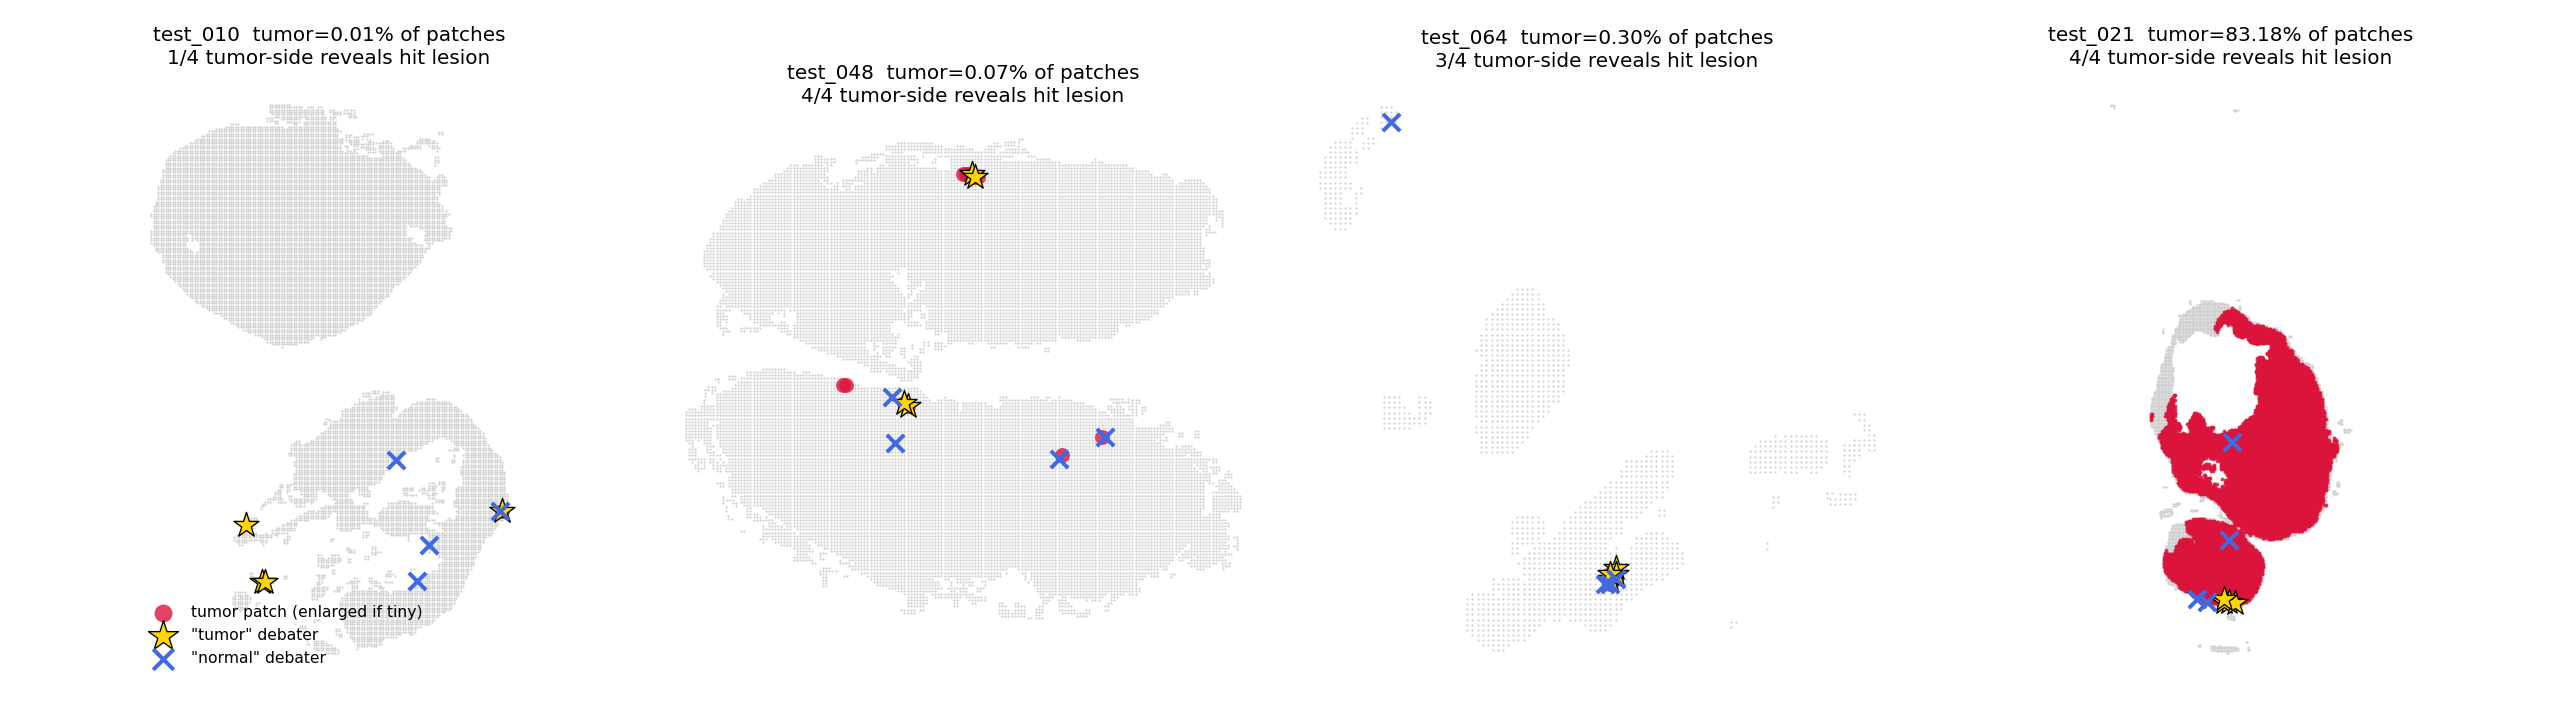
\includegraphics[width=\linewidth]{figs/fig_c16_debate.png}
\caption{Qualitative CAMELYON16 debate: patches revealed by each side. \todo{caption details}}\label{fig:qual}
\end{figure}

%=====================================================================
\section{Discussion and limitations}\label{sec:discussion}
\textbf{Compute.} Our debaters score every item, so debate costs a full read plus a judge; at equal compute it ties full-slide MIL (.94--.97 vs .97). Debate is useful when the party that reads is not the party that decides: a human or expensive model that can inspect $K$ items, with untrusted readers. \textbf{Assumptions.} Soundness requires a competent honest debater (random honest debaters lose). \textbf{Scope.} One pathology encoder per dataset \todo{CONCH on CAMELYON16}; VQA results are single runs \todo{bootstrap CIs}; real WSI agents (e.g.\ GIANT, PathFinder) are not yet audited \todo{}. \textbf{Certification.} Sampling-based certificates~\cite{waudbysmith2024betting,stark2023alpha} offer per-input guarantees against a \emph{trusted} model; combining them with debate-proposed regions is future work.

\section{Conclusion}
Selected-evidence pipelines inherit the trustworthiness of their selector. Across MIL on gigapixel slides and zoom-based VLMs, the selector, not the image, largely determines the answer. When the decider must look at only a few items, letting two untrusted selectors argue before a judge restores accuracy, and the gain grows exactly where selection is needed most: when the evidence is sparse.

\bibliographystyle{abbrvnat}
\bibliography{refs}
\end{document}
